\documentclass[xcolor=dvipsnames,table]{beamer}

\usepackage{latexsym}
\usepackage[utf8]{inputenc}
\usepackage[brazil]{babel}
\usepackage{amssymb}
\usepackage{amsmath}
\usepackage{stmaryrd}
\usepackage{fancybox}
\usepackage{datetime}
\usepackage[T1]{fontenc}
\usepackage{graphicx}
\usepackage{graphics}
\usepackage{url}
\usepackage{algorithmic}
\usepackage{algorithm}
\usepackage{acronym}
\usepackage{array}
\usepackage{multirow}
\usepackage{listings}
\usepackage{animate}

\usepackage{natbib}
\bibliographystyle{ACM-Reference-Format}
\citestyle{acmauthoryear}

\newtheorem{definicao}{Definio}
\newcommand{\tab}{\hspace*{2em}}

\mode<presentation>
{
        \definecolor{colortexto}{RGB}{0,0,0}

        \setbeamertemplate{background canvas}[vertical shading][ bottom=white!10,top=white!10]
        \setbeamercolor{normal text}{fg=colortexto} 

        \usetheme{Warsaw}
}

\title{PondiônsTracker: A framework based on GTFS-RT to identify delays and estimate arrivals dynamically in Public Transportation Network} 

\author{
        Pedro Pongelupe Lopes
}

\institute{Programa de Pós-Graduação em Informática}
\date{\textbf{December 04 2023} }

\logo{
\includegraphics[width=1cm]{images/logoPuc.png}}

\begin{document}

\begin{frame}
        \titlepage
\end{frame}

\begin{frame}{Contents}%[allowframebreaks]{Sumário}
        \tableofcontents[ hideothersubsections]
        %\tableofcontents[currentsection, hideothersubsections]
\end{frame}


\section{Introduction}
\begin{frame}{Introduction}
        \begin{block}{Motivation}
                \begin{itemize}
                        \item Public Transportation Network
                        \item Huge centers 
                        \item GTFS and GTFS-RT specifications
                \end{itemize}
        \end{block}
                \begin{figure}[H]
                        \centering
                        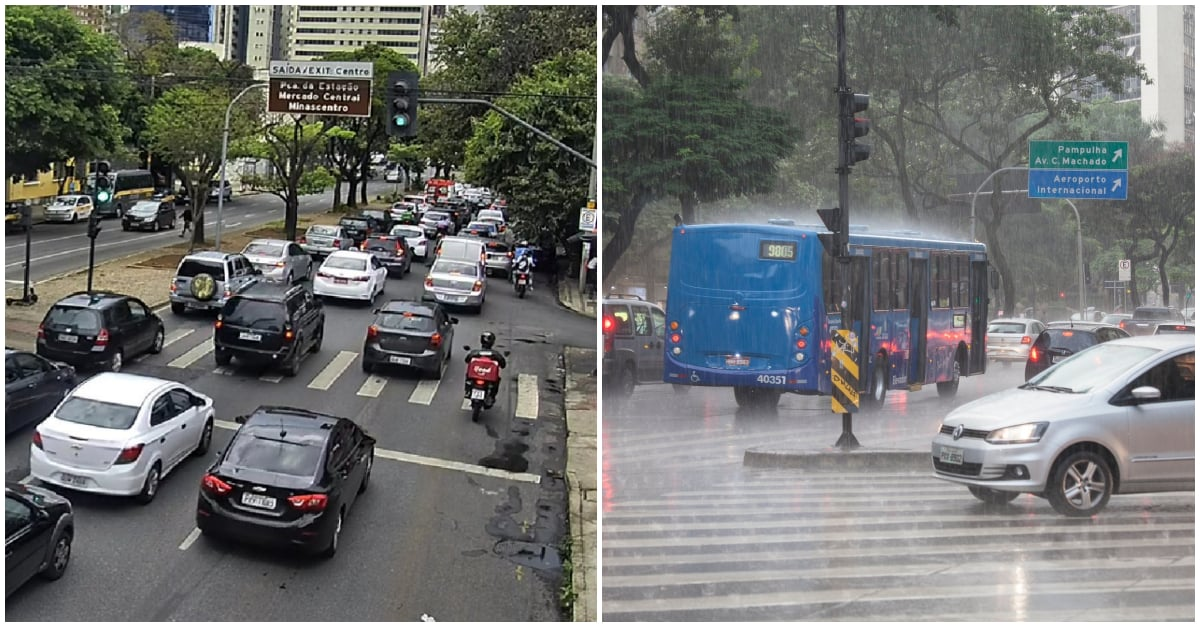
\includegraphics[scale=0.15]{images/chuva-engarrafamento.jpg}
                \end{figure}
\end{frame}

\begin{frame}{Motivation}
        \begin{block}{GTFS-RT Matching Identifiers Issue}
                To work with GTFS-RT, it is \textbf{required} to track vehicles in real-time. But, in some cases, it is not easy to match the identifier between a real-time record and the GTFS static data. In Rome in 2016, this issue was reported by \cite{bigdata}. We still face this issue in Belo Horizonte in 2023.
        \end{block}
\end{frame}

\begin{frame}{Objectives}
        \begin{block}{Main Objective}
                \begin{itemize}
                        \item Proposing and validating PondiônsTracker
                \end{itemize}
        \end{block}
        \begin{block}{Specific Objectives}
                \begin{itemize}
                        \item Collecting data from the real-time API and combining with the GTFS
                        \item Understanding if Belo Horizonte's delays are spatial and temporal dependent by analyzing delays among bus stops
                        \item Comparing the arrival times defined at the GTFS with the arrival times generated by \textit{PondiônsTracker}.
                \end{itemize}
        \end{block}
\end{frame}


\section{Theoretical Reference}
\begin{frame}{Theoretical Reference}
        \begin{block}{Main Ideas}
                \begin{itemize}
                        \item Smart Cities
                        \item Urban Computing
                        \item Human Mobility
                        \item Graphs and Complex Network
                \end{itemize}
        \end{block}
\end{frame}

\begin{frame}{Complex Networks and Graphs}
        \begin{columns}
                \column{0.5\textwidth}  		
                \begin{block}{Definition}
                        \citealp{Bacciu_2020} state that "a graph has a compositional nature, being 
                        a compound of atomic information pieces and a relational nature, as the links
                        defining its structure denote relationships between the linked entities".

                        \begin{itemize}
                                \item \textit{$g = (V_g, E_g, X_g, A_g)$}
                        \end{itemize}
                \end{block}
                \column{0.5\textwidth}
                \centering
                \begin{figure}[H]
                        \centering
                        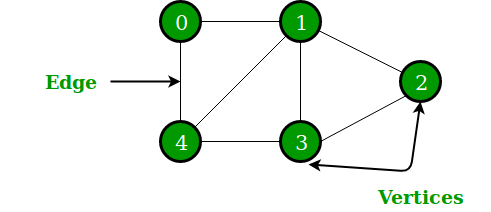
\includegraphics[scale=0.35]{images/undirectedgraph.png}
                        \caption{Example of an undirected graph}
                \end{figure}
        \end{columns}
\end{frame}
\begin{frame}{Public Transportation Network as a Complex Network}
        \begin{figure}[H]
                \centering
                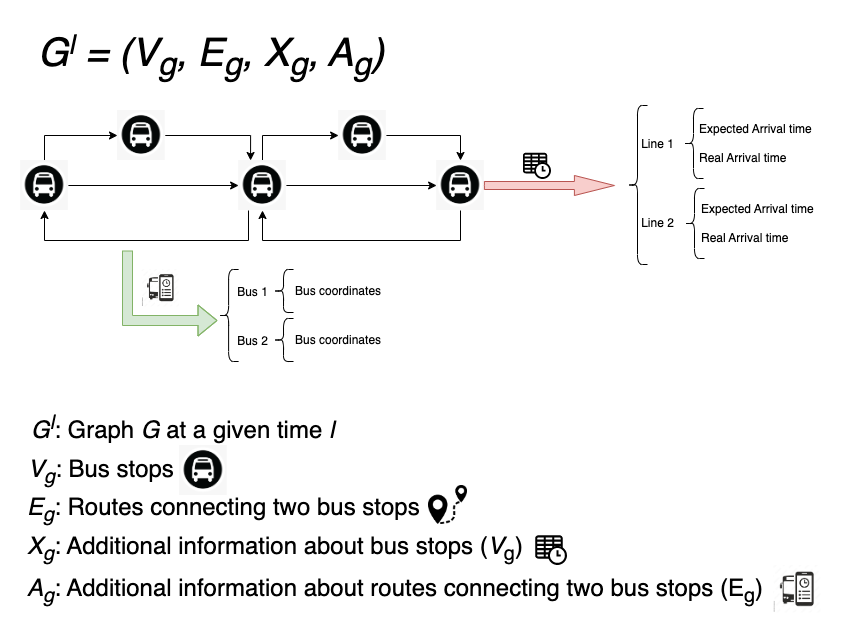
\includegraphics[scale=0.3]{images/final_graph.png}
                \caption{Delimiting Trips into Routes}
        \end{figure}
\end{frame}


\section{Related Work}
\begin{frame}{Related Work}
        \begin{block}{Main Ideas}
                \begin{itemize}
                        \item GTFS-RT matching identifiers issue 
                        \item Public Transportation Network as a complex network
                        \item Delay analysis
                        \item Algorithm outline after monitoring vehicles in real-time
                \end{itemize}
        \end{block}
\end{frame}

\section{PondiônsTracker}
\subsection{Architecture and Entities}
\begin{frame}{PondiônsTracker}
        \begin{block}{Overview}
                \textit{PondiônsTracker}\footnote{Available at \url{https://github.com/Pongelupe/PondionsTracker/}} 
                is a framework to enrich
                GTFS data with real-time data. 
                The name \textit{PondiônsTracker} is a small gag from the sonority of the expression{ \em 'bus stop'}
                when pronounced in Portuguese with the accent from Minas Gerais.
        \end{block}
\end{frame}
\begin{frame}{PondiônsTracker's Architecture}
        \begin{figure}[H]
                \centering
                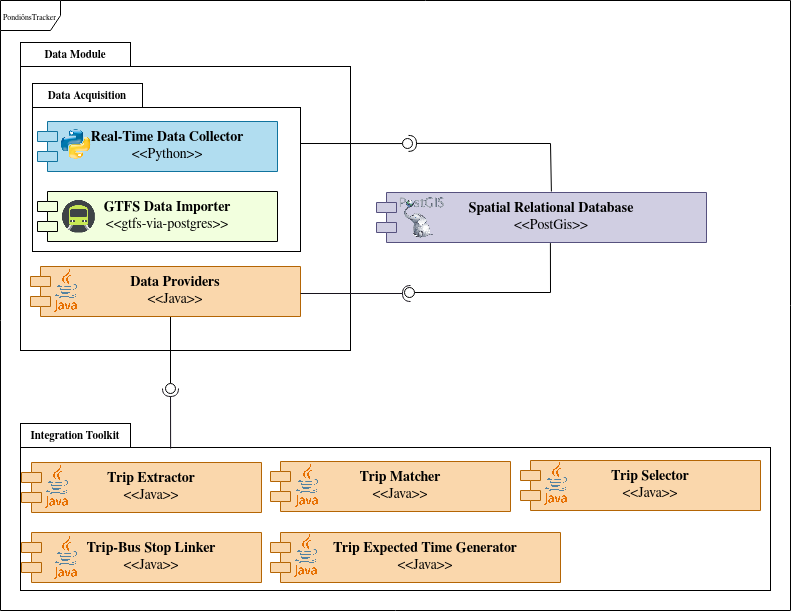
\includegraphics[scale=0.3]{images/arq-pondionstracker.drawio.png}
                \caption{\textit{PondiônsTracker}'s architecture diagram}
        \end{figure}
\end{frame}
%\begin{frame}{PondiônsTracker's Entities}
%       \begin{figure}[H]
%               \centering
%               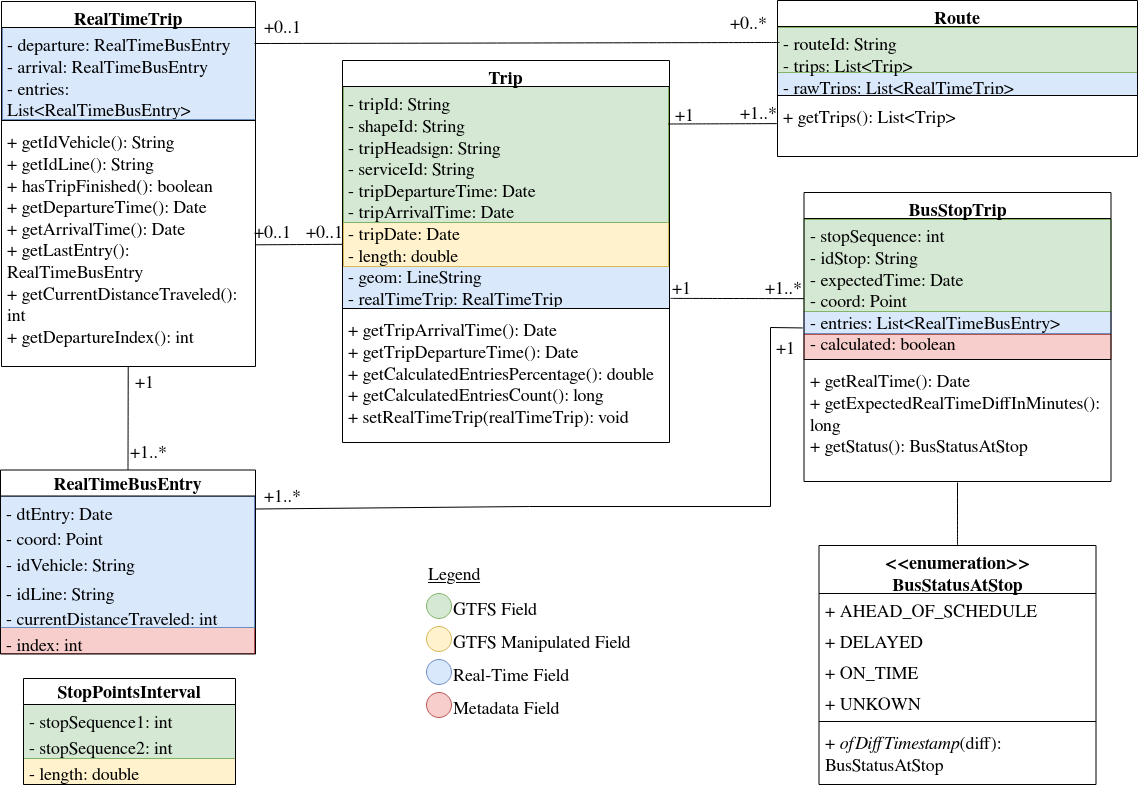
\includegraphics[scale=0.23]{images/entitiesCD.png}
%               \caption{\textit{PondiônsTracker}'s architecture diagram}
%       \end{figure}
%\end{frame}

\subsection{Data Module}
\begin{frame}{Data Module Overview}
        \begin{figure}[H]
                \centering
                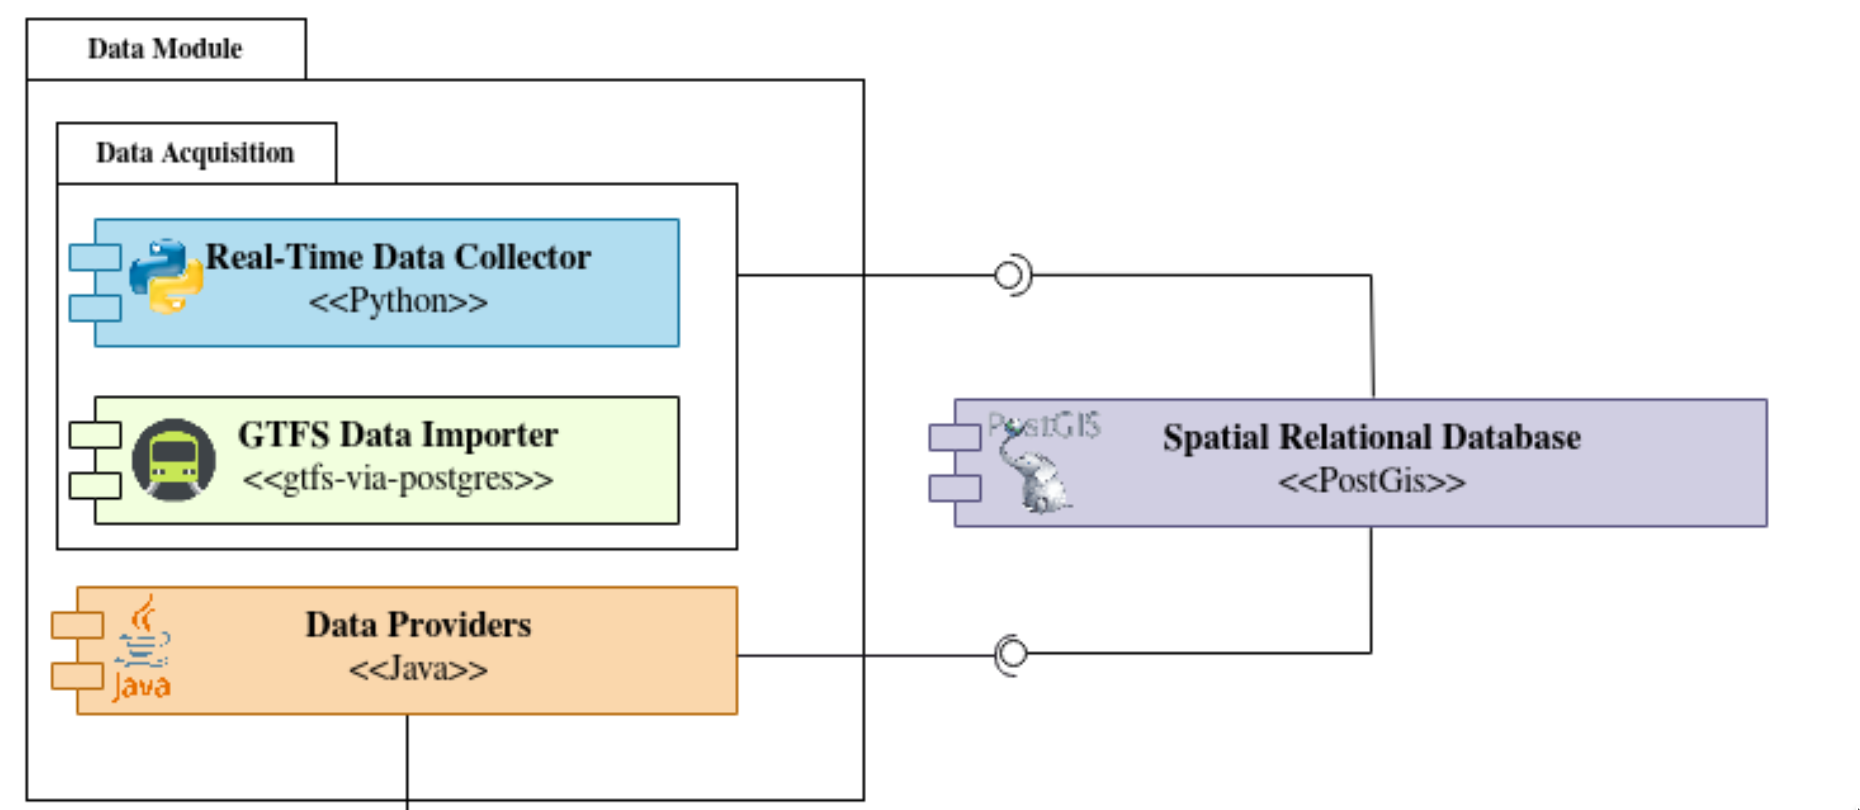
\includegraphics[width=\textwidth]{images/datamodule.png}
        \end{figure}
\end{frame}


\begin{frame}{Data Acquisition - GTFS Data Importer}
        \begin{figure}
                \centering
                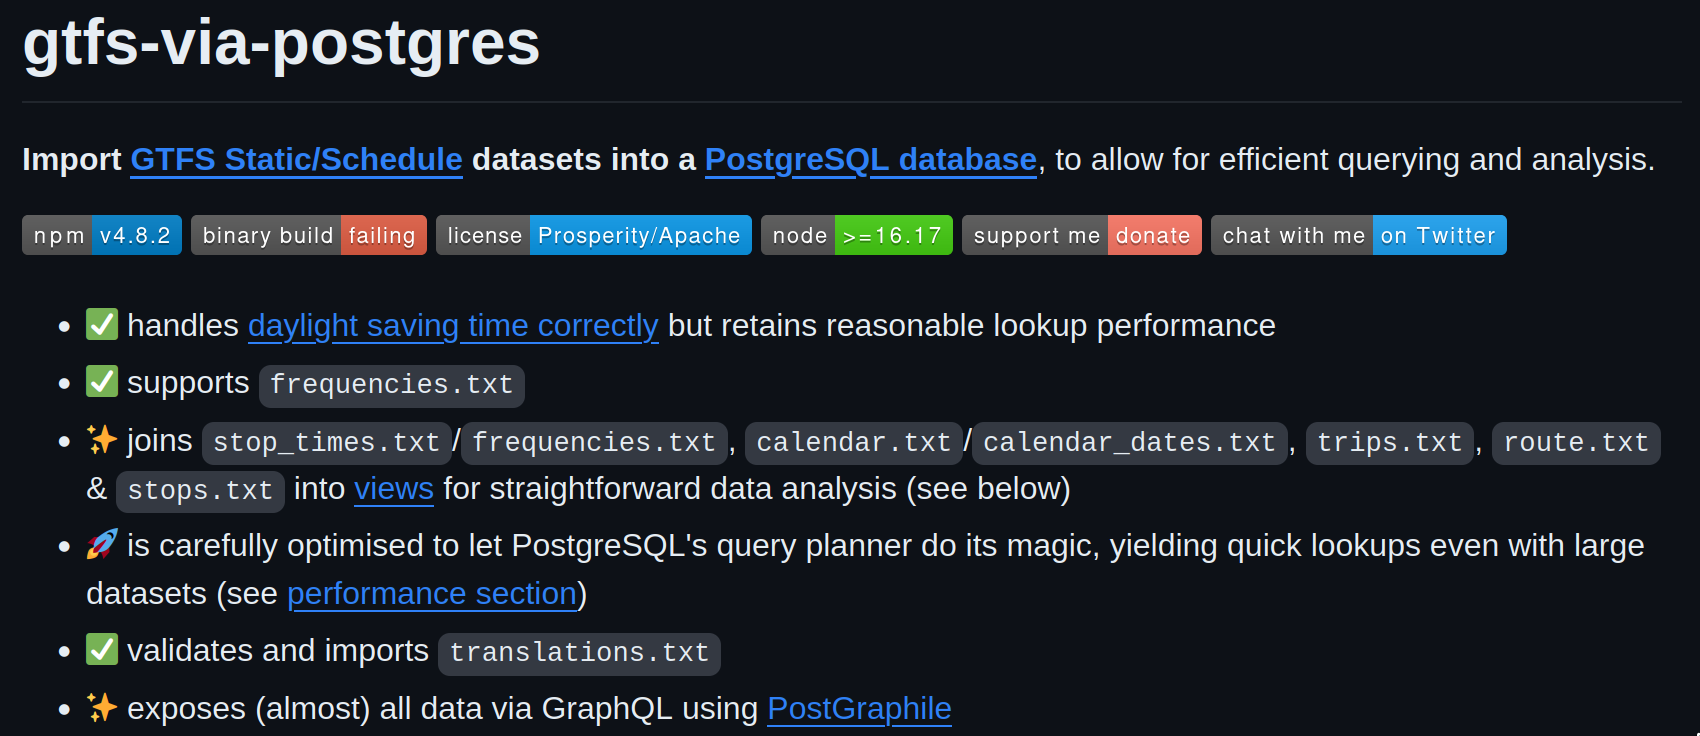
\includegraphics[width=\textwidth]{images/GTFS-via-postgres.png}
                \caption{\textit{gtfs-via-postgres}'s README}
        \end{figure}
\end{frame}


\begin{frame}{Data Acquisition - Real-Time Data Collector}
        \begin{block}{Considerations}
                This component incorporates the data 
                from real-time traffic \textit{API} provided by some external source.
        \end{block}
        \begin{figure}[H]
                \centering
                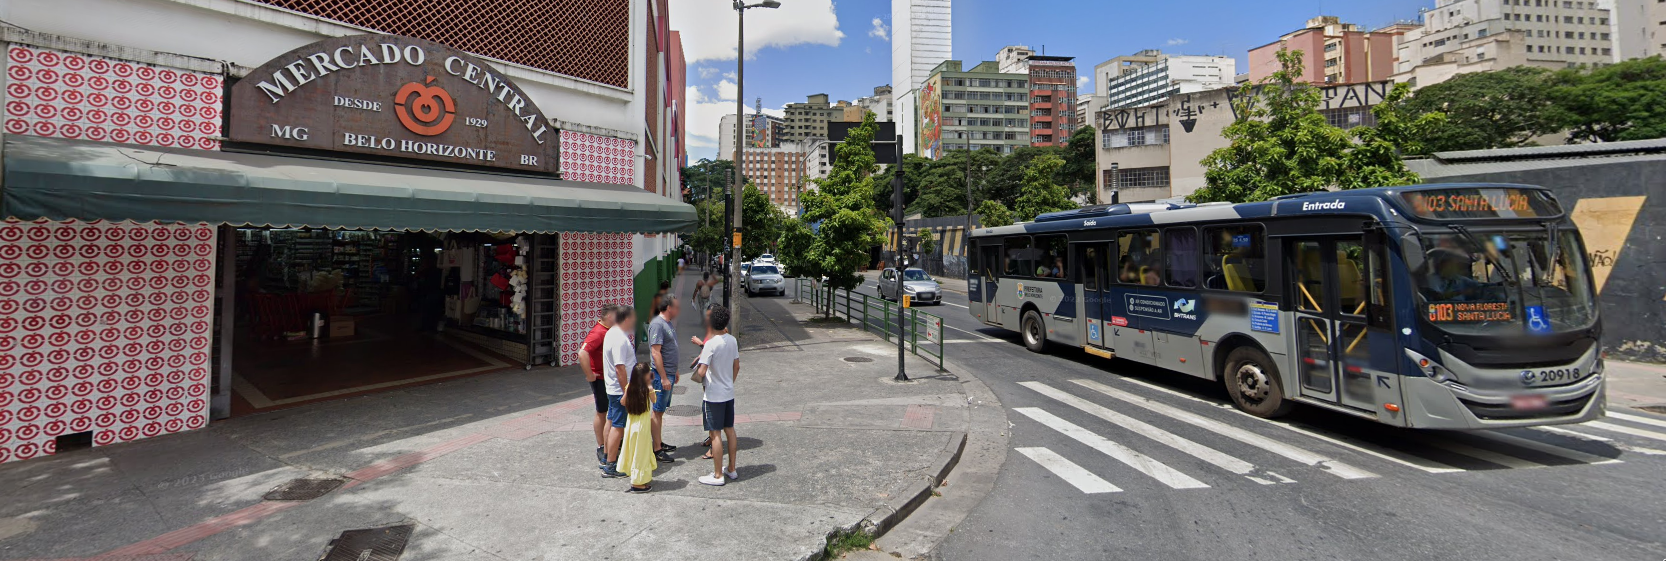
\includegraphics[width=\textwidth]{images/entry_mercado.png}
        \end{figure}
\end{frame}
\begin{frame}{Data Providers}
        \begin{figure}[H]
                \centering
                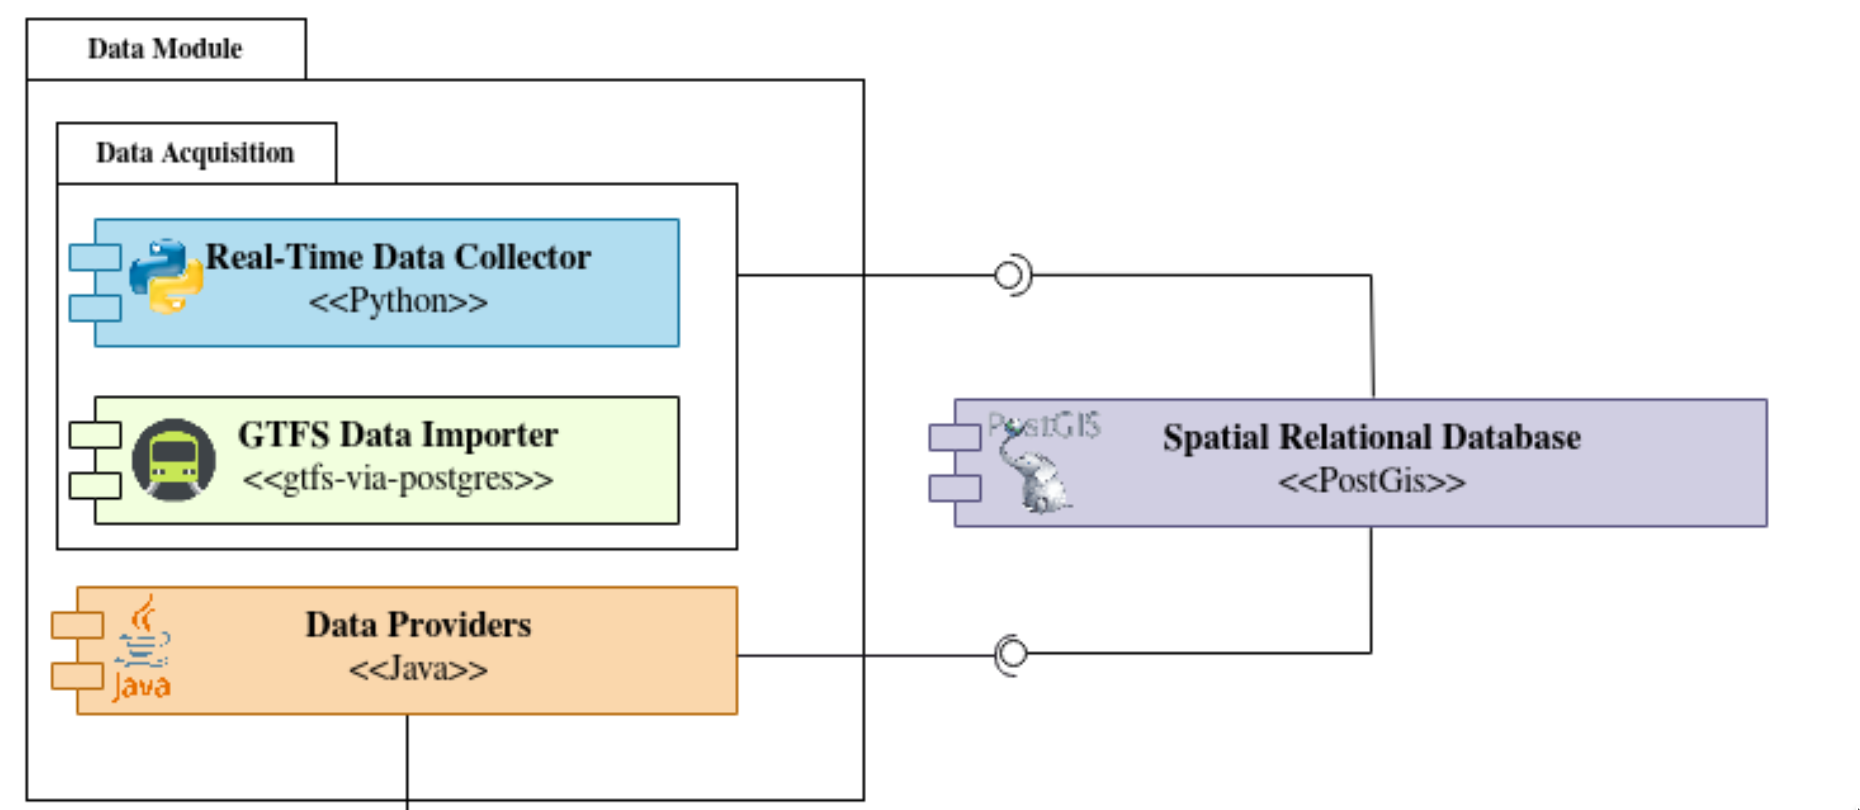
\includegraphics[width=\textwidth]{images/datamodule.png}
        \end{figure}
\end{frame}

\begin{frame}{Data Providers}
        \begin{figure}[H]
                \centering
                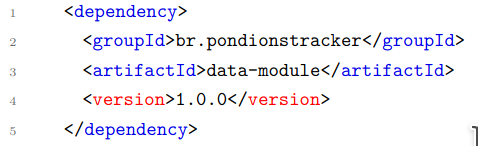
\includegraphics[scale=0.45]{images/mddatamodule.png}
                \caption{\textit{DataModule}'s maven dependency}
        \end{figure}
\end{frame}

\subsection{Integration Module}
\begin{frame}{Integration Module}
        \begin{figure}[H]
                \centering
                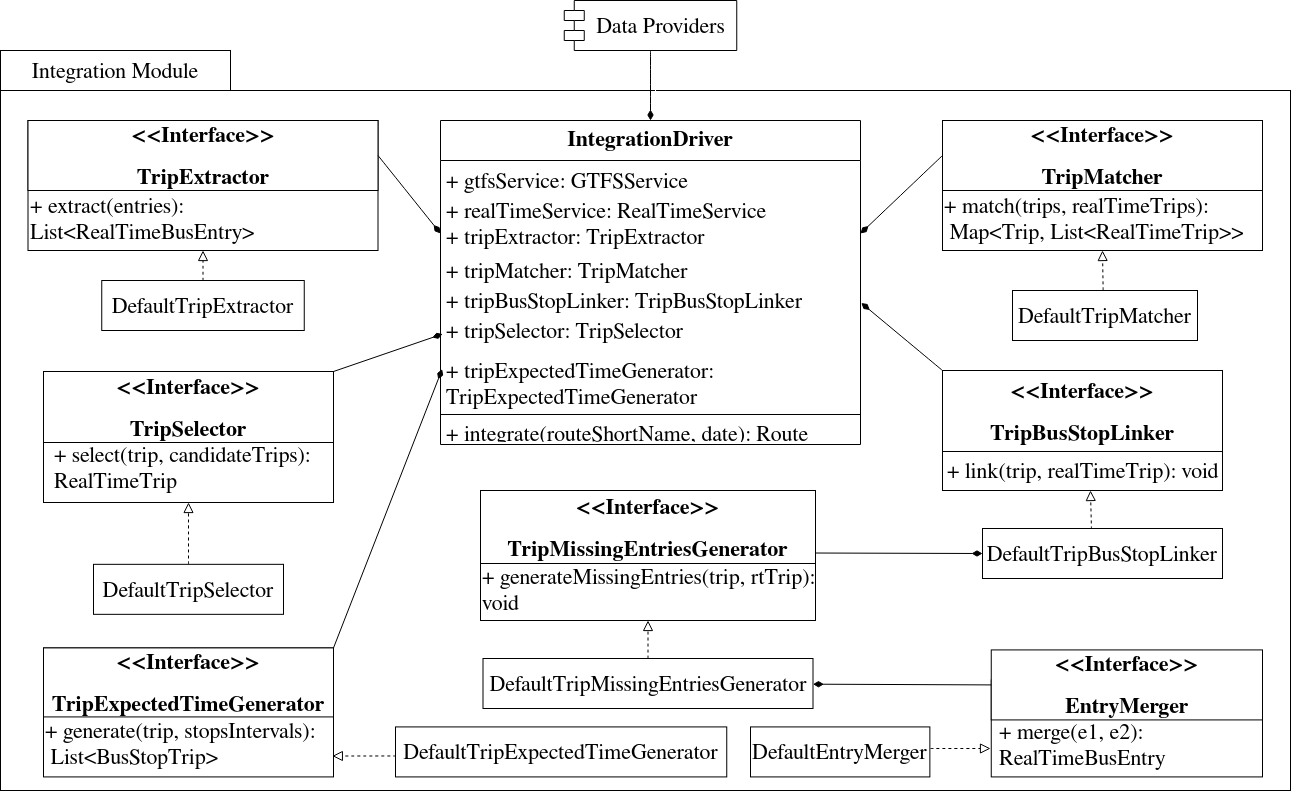
\includegraphics[scale=.205]{images/integrationModuleCD.png}
                \caption{Integration Module Class Diagram}
        \end{figure}
\end{frame}
\begin{frame}{Integration Driver}
        \begin{figure}[H]
                \centering
                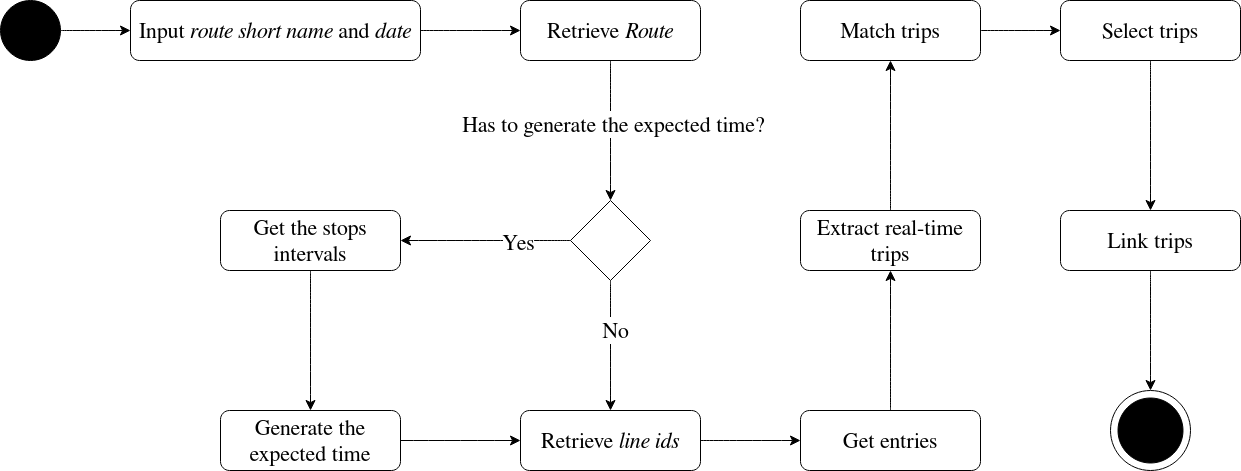
\includegraphics[width = \textwidth]{images/integrationDriverAD.drawio.png}
                \caption{Integration Driver Activity Diagram}
        \end{figure}
\end{frame}
\begin{frame}{Integration Driver - 1st Step}
        \begin{figure}[H]
                \centering
                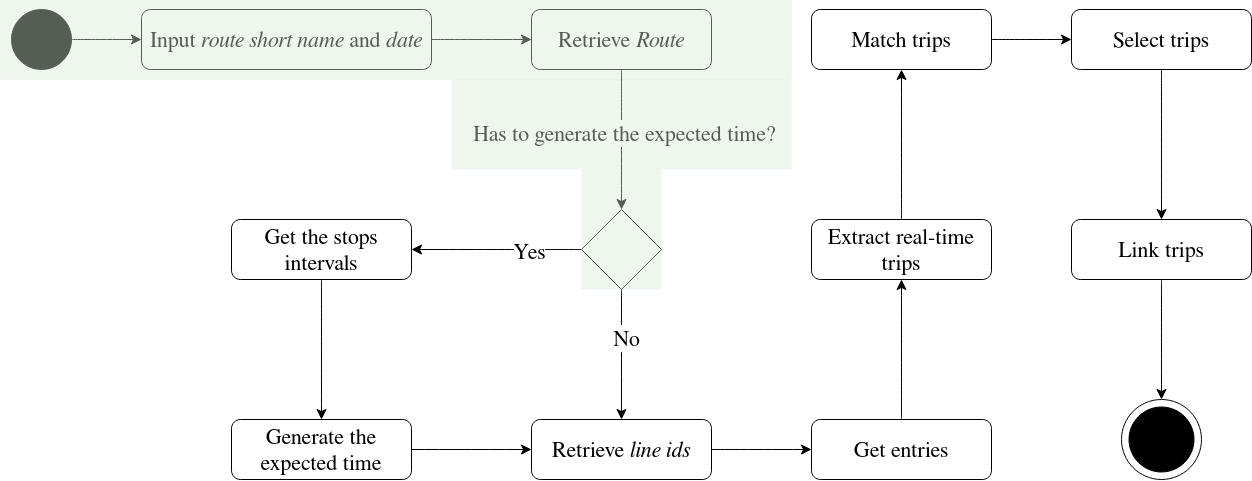
\includegraphics[width = \textwidth]{images/integrationDriverAD(1st_step).png}
                \caption{Integration Driver Activity Diagram}
        \end{figure}
\end{frame}
\begin{frame}{Has to generate the expected time?}
        \begin{figure}[H]
                \centering
                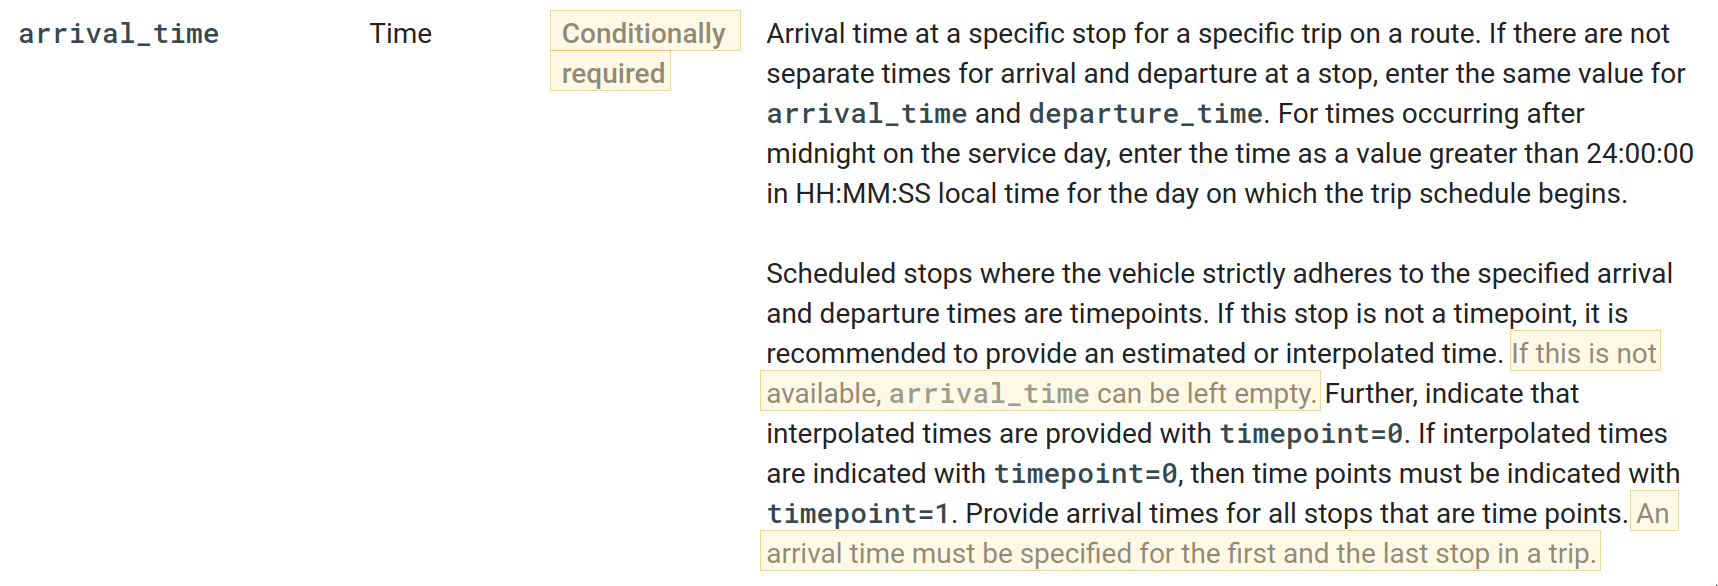
\includegraphics[width = \textwidth]{images/arrival_time_def.png}
                \caption{$arrival\_time$ definition from $stop\_times.txt$}
        \end{figure}
\end{frame}
\begin{frame}{Integration Driver - 2nd Step*}
        \begin{figure}[H]
                \centering
                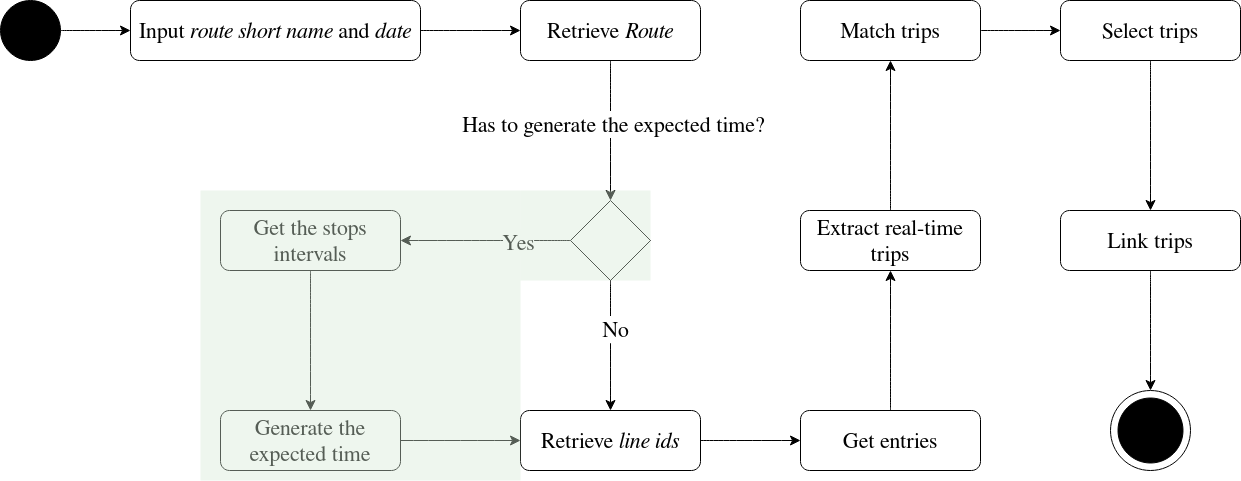
\includegraphics[width = \textwidth]{images/integrationDriverAD(2nd_step).png}
                \caption{Integration Driver Activity Diagram}
        \end{figure}
\end{frame}

\begin{frame}{Integration Driver - 2nd Step*}
        \begin{block}{Overview}
                \begin{enumerate}
                        \item Get the stop intervals
                        \item Generate the expected time using \textit{TripExpectedTimeGenerator}
                \end{enumerate}
        \end{block}
        \begin{figure}[H]
                \centering
                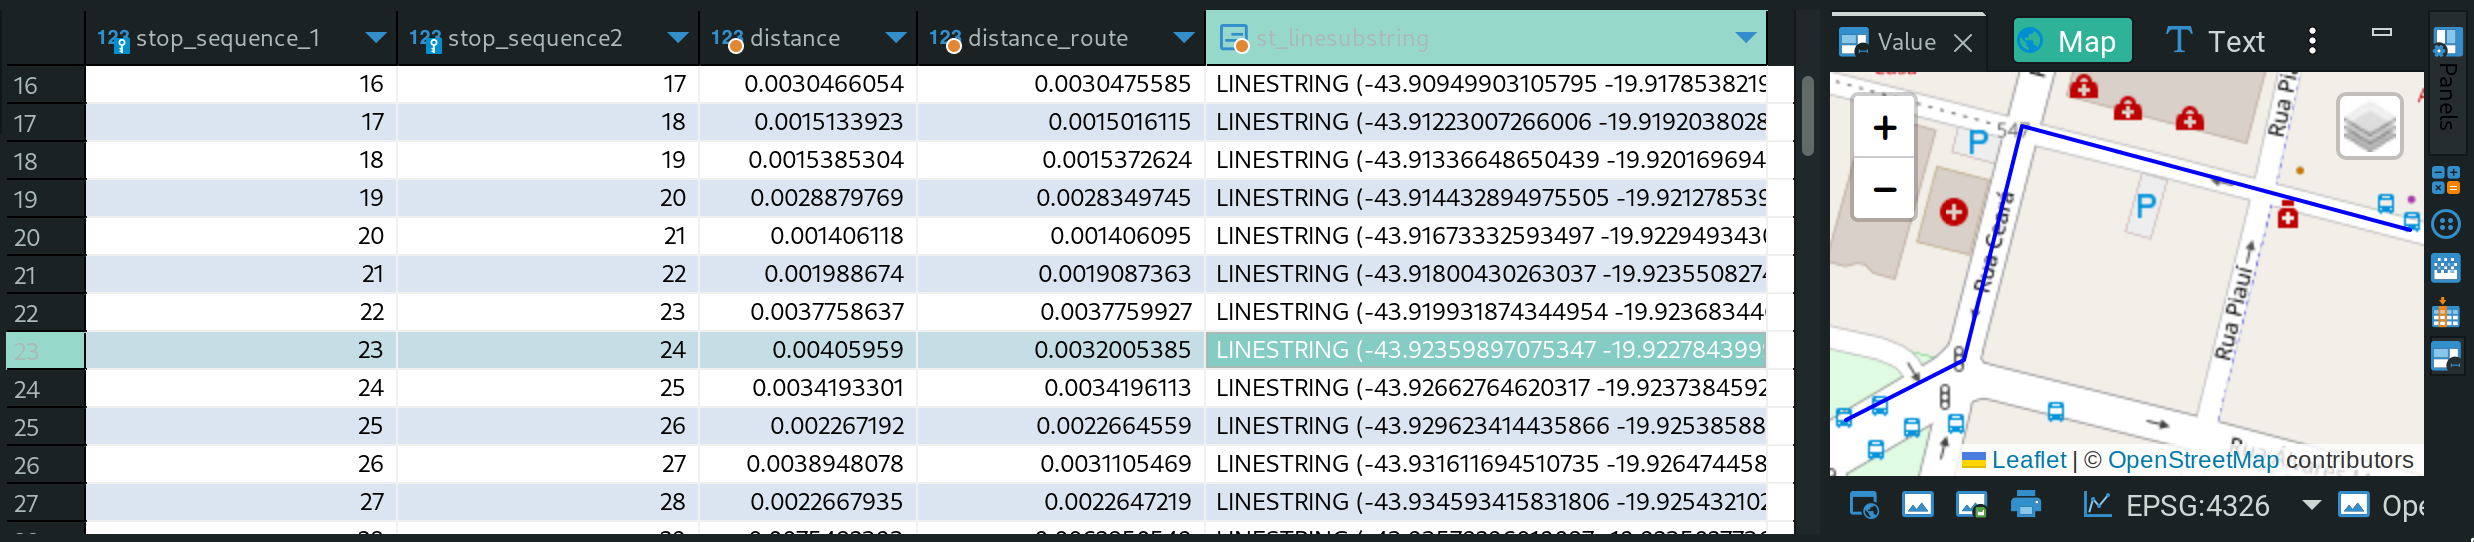
\includegraphics[width = \textwidth]{images/couplepoints.png}
                \caption{Example of bus stop couples and their distance}
        \end{figure}
\end{frame}

\begin{frame}{\textit{TripExpectedTimeGenerator}}
        \begin{block}{Default Implementation key ideas}
                \begin{itemize}
                        \item Stop times are incremental in the trip
                                and are incremented at each stop.
                        \item $arrival\_time \rightarrow departure\_time$
                        \item The bus {\em should} travel the trip in average speed
                        \item Minor deviations to the original $departure\_time$
                \end{itemize}
        \end{block}
\end{frame}

\begin{frame}{Integration Driver - 3rd Step}
        \begin{figure}[H]
                \centering
                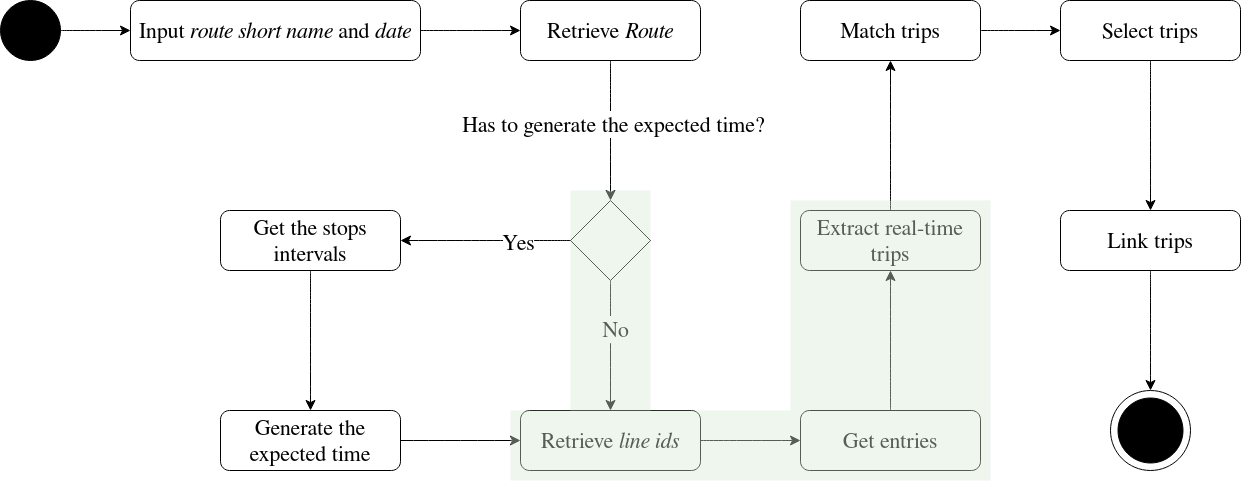
\includegraphics[width = \textwidth]{images/integrationDriverAD(3rd_step).png}
                \caption{Integration Driver Activity Diagram}
        \end{figure}
\end{frame}

\begin{frame}{Integration Driver - 4th Step}
        \begin{figure}[H]
                \centering
                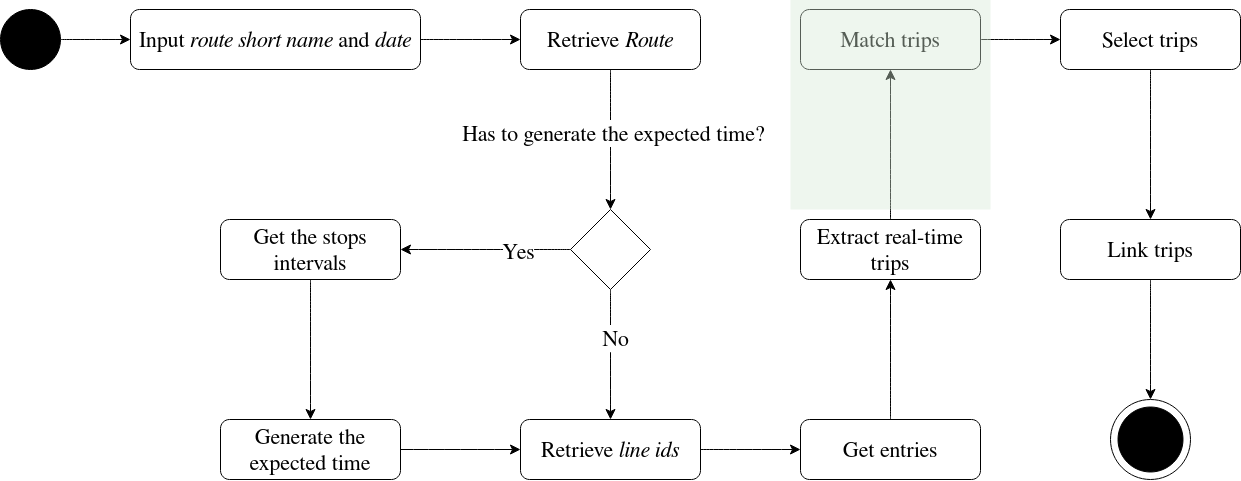
\includegraphics[width = \textwidth]{images/integrationDriverAD(4th_step).png}
                \caption{Integration Driver Activity Diagram}
        \end{figure}
\end{frame}
\begin{frame}{\textit{TripMatcher}}
        \begin{block}{Default Implementation key ideas}
                \begin{itemize}
                        \item Linking static data to real-time data
                        \item Compare schedules using padding
                        \item For a \textbf{scheduled trip} there are many \textbf{candidate trips}
                \end{itemize}
        \end{block}
\end{frame}

\begin{frame}{Integration Driver - 5th Step}
        \begin{figure}[H]
                \centering
                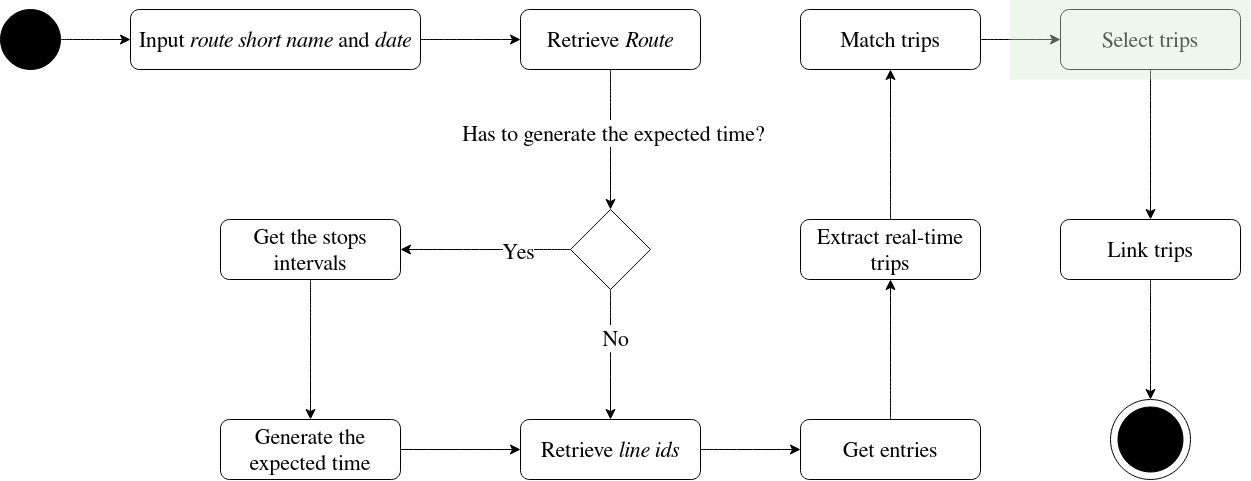
\includegraphics[width = \textwidth]{images/integrationDriverAD(5th_step).png}
                \caption{Integration Driver Activity Diagram}
        \end{figure}
\end{frame}

\begin{frame}{Integration Driver - 6th Step}
        \begin{figure}[H]
                \centering
                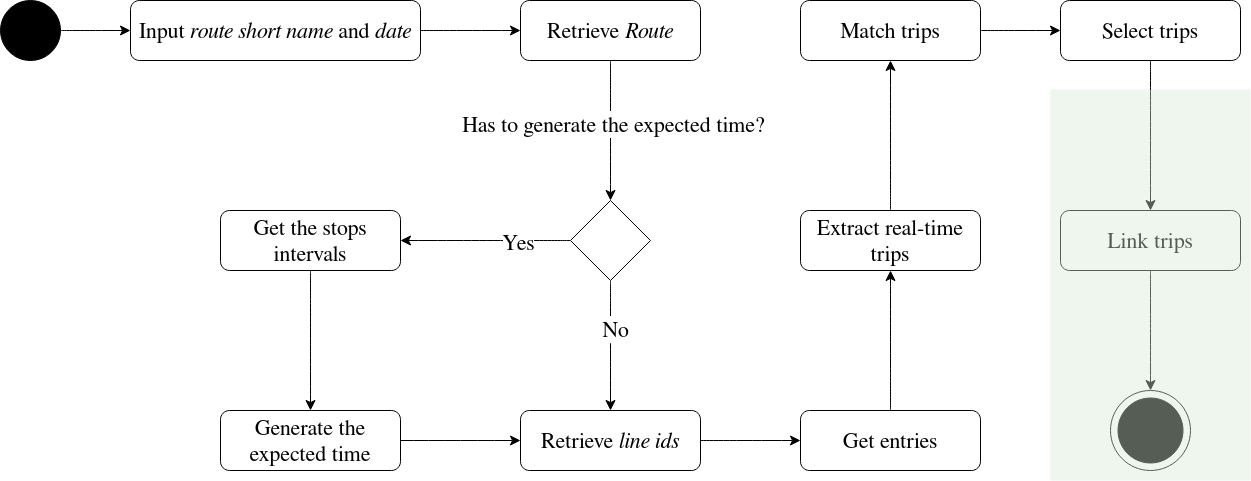
\includegraphics[width = \textwidth]{images/integrationDriverAD(6th_step).png}
                \caption{Integration Driver Activity Diagram}
        \end{figure}
\end{frame}
\begin{frame}{\textit{TripBusStopLinker}}
        \begin{block}{Default Implementation Premises}
                \begin{itemize}
                        \item $RealTimeTrip$ have
                                been \textbf{around} every bus stop from their route
                        \item What is the concept of an entry to be \textbf{around} a bus stop?
                        \item Distance threshold $d_t$
                \end{itemize}
        \end{block}
        \begin{figure}[H]
                \centering
                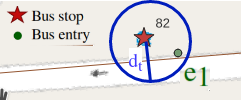
\includegraphics[scale=.6]{images/entriesDT.drawio.png}
                \caption{Entries and $d_t$ representations}
        \end{figure}
\end{frame}
\begin{frame}{\textit{TripBusStopLinker}}
        \begin{block}{Default Implementation key ideas}
                Iterate over $Trip$'s $busStopSequence$
                and for each bus stop $s_x$ it is searched for all the \textbf{valid} entries within $d_t$*, then scanning the $RealTimeTrip$'s $entries$ set.
        \end{block}
        \begin{block}{Relationship between Entries and Bus Stops}
                An entry $e$ to a bus stop $s_x$:
                \begin{enumerate}
                        \item An entry $e$ can be associated with only one $s_x$
                        \item A $s_x$ can be related to more than one entry $e$
                        \item A $s_x$ can be related to \textbf{zero entries}
                \end{enumerate}
        \end{block}
\end{frame}
\begin{frame}{Empty Set of Entries}
        \begin{block}{Why do we have an empty set?}
                This does not imply that the bus has not been around a stop on the trip, 
                it might be only a GPS positioning error. For example, if a bus is at a
                certain speed, it passes by a bus stop without stopping because there
                is no boarding or landing at that given stop.
        \end{block}
        \begin{figure}[h]
                \centering
                \caption{A bus stop with no entries related}
                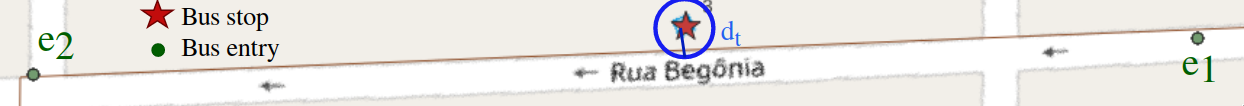
\includegraphics[width=\textwidth]{images/9202_empty_set.png}
        \end{figure}
\end{frame}
\begin{frame}{\textit{TripMissingEntriesGenerator}}
        \begin{block}{Default Implementation Overview}
                \begin{itemize}
                        \item Generate an artificial entry by merging a couple of entry
                        \item The \textit{EntryMerger} is the component
                                in charge of merging two entries
                                \begin{itemize}
                                        \item \textbf{Linear Interpolation}
                                \end{itemize}
                \end{itemize}
        \end{block}
        \begin{figure}[h]
                \centering
                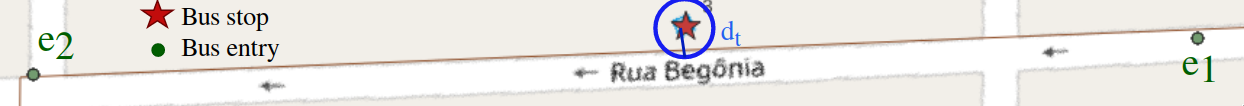
\includegraphics[width=\textwidth]{images/9202_empty_set.png}
        \end{figure}
\end{frame}
\begin{frame}{\textit{TripMissingEntriesGenerator}}
        \begin{columns}
                \column{0.5\textwidth} 
                \begin{block}{Which entries are going to be merged?}
                        \begin{itemize}
                                \item Defining an interval of candidates entries
                                \item {\em Lower Bound Entry} and {\em Upper Bound Entry}
                                \item The closest entries to the bus stop from each side of the interval
                        \end{itemize}
                \end{block}
                \column{0.5\textwidth}
                \begin{figure}[h]
                        \centering
                        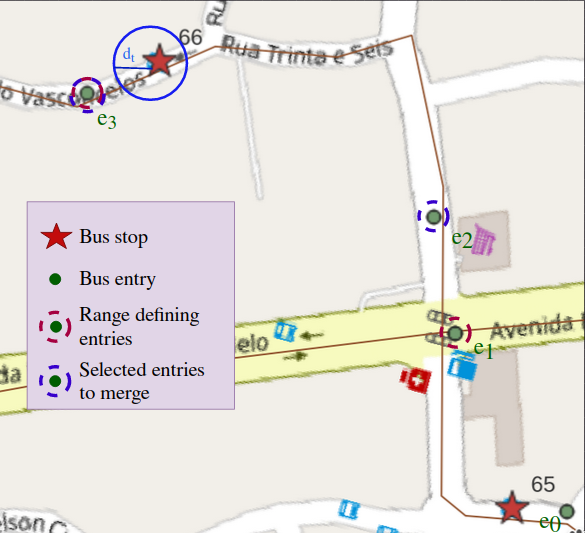
\includegraphics[width=\textwidth]{images/9202_hard.png}
                \end{figure}
        \end{columns}
\end{frame}

\begin{frame}{Integration Driver}
        \begin{figure}[H]
                \centering
                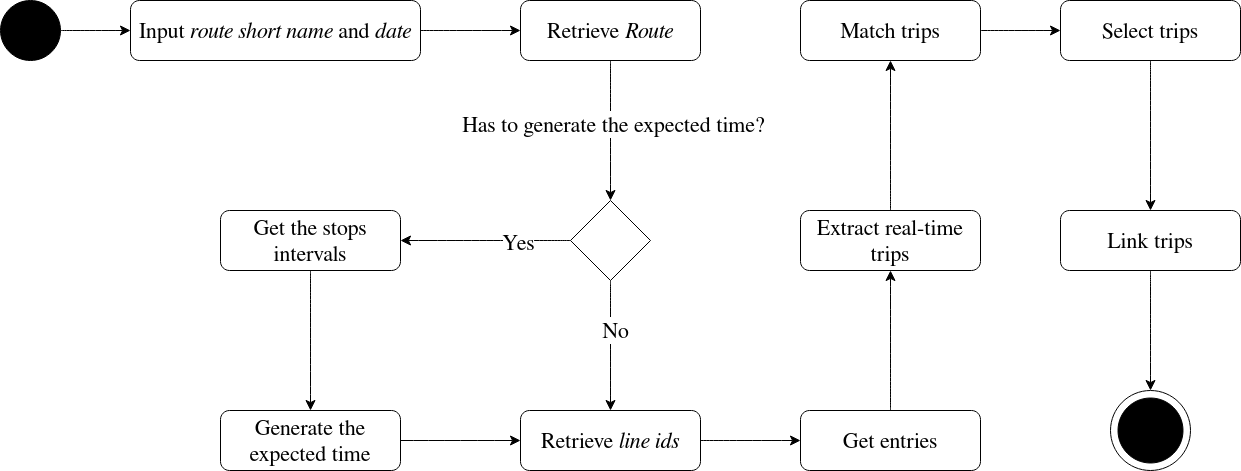
\includegraphics[width = \textwidth]{images/integrationDriverAD.drawio.png}
                \caption{Integration Driver Activity Diagram}
        \end{figure}
\end{frame}
\begin{frame}{Integration Module}
        \begin{figure}[H]
                \centering
                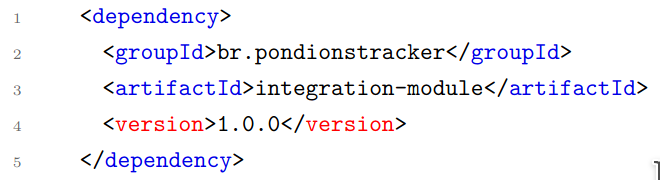
\includegraphics[scale=0.45]{images/mdIntegrationModule.png}
                \caption{\textit{IntegrationModule}'s maven dependency}
        \end{figure}
\end{frame}

\subsection{PondiônsTracker-BH}
\begin{frame}{PondiônsTracker-BH}
        \begin{block}{Overview}
                \textit{PondiônsTracker-BH}\footnote{Available at \url{https://github.com/Pongelupe/PondionsTracker-BH}} is a \textit{PondiônsTracker}'s specialization created to
                deal with Belo Horizonte's Public Transportation Network particularities. So, we have implemented our own \textit{Real-Time Data collector}, and we have overwritten the method \textit{getIdsLineByRouteId} from the 
                \textit{RealTimeService}.
                \begin{itemize}
                        \item $BHTrans \rightarrow GTFS$
                        \item $Transfacil \rightarrow Traffic\ API$
                \end{itemize}
        \end{block}
\end{frame}
\begin{frame}{Belo Horizonte’s RealTimeService}
        \begin{block}{\textit{BHRealTimeService}}
                \textit{BHRealTimeService} {\em extends} \textit{DefaultRealTimeService} and overrides \textit{getIdsLineByRouteId} method. There is a \textbf{one-to-many} relationship between the GTFS and the real-time data.
        \end{block}
\end{frame}

\section{Results}
\begin{frame}{Workload Overview}
        \begin{columns}
                \column{0.5\textwidth} 
                \begin{block}{Workload}
                        \begin{itemize}
                                \item Data collected for 11 days straight in August 2023 
                                \item 30 Gigabytes 
                        \end{itemize}
                \end{block}
                \column{0.5\textwidth}
                \begin{figure}[h]
                        \centering
                        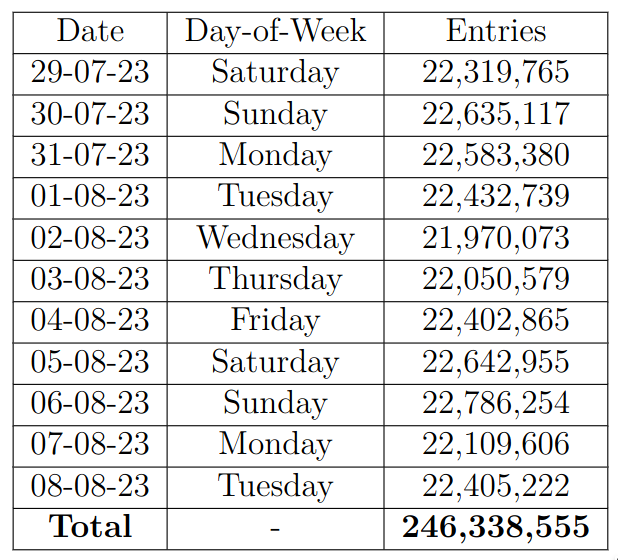
\includegraphics[width=\textwidth]{images/workload.png}
                \end{figure}
        \end{columns}
\end{frame}
\subsection{Schedule Analysis}
\begin{frame}{Schedule Analysis}
        \begin{block}{\textit{Schedule-Filled Percentage}}
                \textit{Schedule-Filled Percentage} = \textbf{Matched Trips} / \textbf{Scheduled Trips}
                \begin{itemize}
                        \item \textbf{Total}: 156,628 / 205,884 = 76.08\% 
                        \item \textbf{Weekdays}: 118,559 / 159,418 = 74.37\% 
                        \item \textbf{Saturdays}: 22,796 / 28,200 = 80.84\% 
                        \item \textbf{Sundays}: 15,273 / 18,266 = 83.61\% 
                \end{itemize}
        \end{block}
\end{frame}
\begin{frame}{Schedule Analysis - Schedule Deviations}
        \begin{block}{Schedule Deviations}
                Regarding the real-time API, there are collected trips which were not defined at Belo Horizonte's GTFS.
        \end{block}
        \begin{block}{\textit{82 - Estação São Gabriel / Savassi Via Hospitais}}
                On Sundays, the GTFS does not schedule any trip for route $82$,
                but the API provided
                entries regarding this route twice during the period observed.
        \end{block}
\end{frame}

\subsection{Delay Analysis}
\begin{frame}{Delay Analysis}
        \begin{block}{Delay Notation}
                \begin{itemize}
                        \item \textbf{Delay}: $\geqslant$ 1 minute after
                        \item \textbf{Ahead-of-Schedule}: $\geqslant$ 1 minute before
                        \item \textbf{On time}: $\leqslant$ 59 seconds after OR $\leqslant$ 59 seconds before
                \end{itemize}
        \end{block}
        \begin{figure}[H]
                \centering
                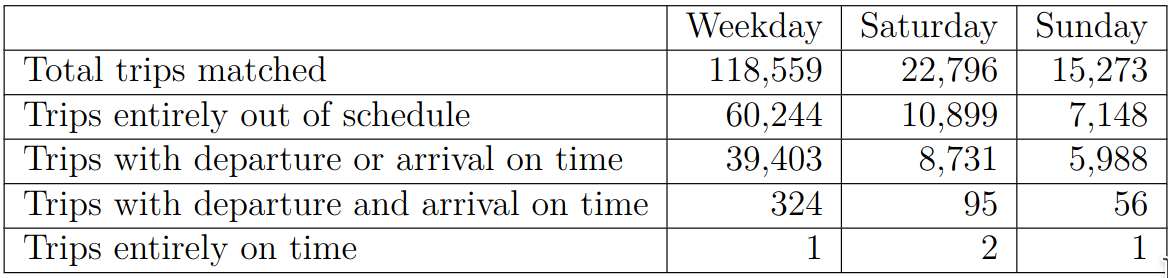
\includegraphics[width=\textwidth]{images/delays_detailed.png}
                \caption{Delays detailed in whole Public Transportation Network scale}
        \end{figure}
\end{frame}
\begin{frame}{Delay Analysis}
        \begin{block}{\textit{331 - Estação Barreiro/Conjunto Antonio Teixeira Dias Via Upa}}
             Has 32 bus stops, representing a length of almost 9 kilometers.
                \begin{enumerate}
                        \item Jul. 29 15:30:00 - 15:56:27 $\longrightarrow$ Jul. 29 15:30:03 - 15:57:03
                        \item Jul. 30 08:20:00 - 08:46:27 $\longrightarrow$ Jul. 30 08:20:31 - 08:46:15
                        \item Aug. 04 05:40:00 - 06:06:27 $\longrightarrow$ Aug. 04 05:40:30 - 06:06:00
                        \item Aug. 05 17:10:00 - 17:36:27 $\longrightarrow$ Aug. 05 17:10:45 - 17:36:49
                \end{enumerate}
        \end{block}
\end{frame}
\begin{frame}{Delay Analysis}
        \begin{columns}
                \column{0.5\textwidth}  		
                \begin{block}{Distribution of each status over the network}
                        \begin{itemize}
                                \item \textbf{Delay}: 89.8\% 
                                \item \textbf{Ahead-of-Schedule}: 6.9\% 
                                \item \textbf{On time}: 3.3\%
                        \end{itemize}
                \end{block}
                \column{0.5\textwidth}
                \centering
                \begin{block}{\textbf{Attention!}}
                        The predominance of $DELAYED$ in the Public Transportation Network \textbf{does not imply} that the network is not working
nor completely stopped!
                \end{block}
        \end{columns}
\end{frame}
\begin{frame}{Delay Analysis}
                \begin{block}{Delays distribution over the network}
                        \begin{itemize}
                                \item Bus Stop
                                \item Trips
                        \end{itemize}
                \end{block}
        \begin{figure}[H]
                \centering
                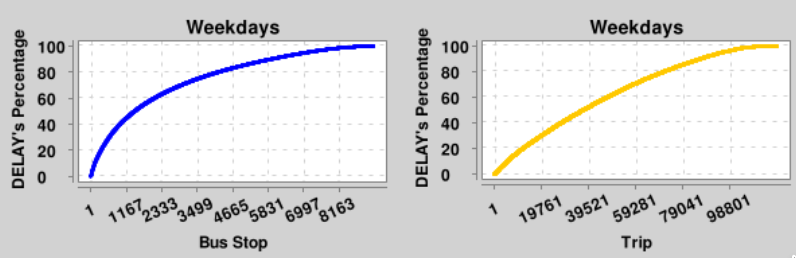
\includegraphics[width=\textwidth]{images/delays_distribution.png}
                \caption{$DELAY$s Distribution: Bus Stop and Trip}
        \end{figure}
\end{frame}
\begin{frame}{Delay Analysis}
        \begin{columns}
                \column{0.5\textwidth}  		
                \begin{figure}[H]
                        \centering
                        \caption{300 Most Delayed Stops}
                        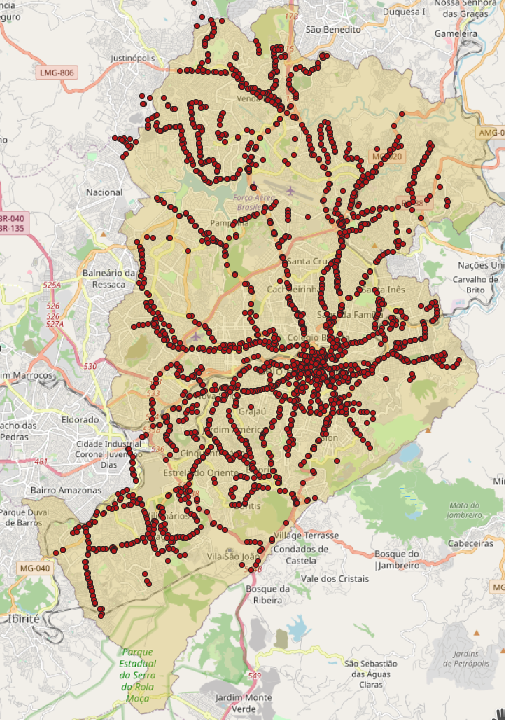
\includegraphics[height=5cm, keepaspectratio]{images/mostDelayedStops.png}
                \end{figure}
                \column{0.5\textwidth}
                \begin{figure}[t]
                        \centering
                        \caption{Fragment of the 50 Most Delayed Stops }
                        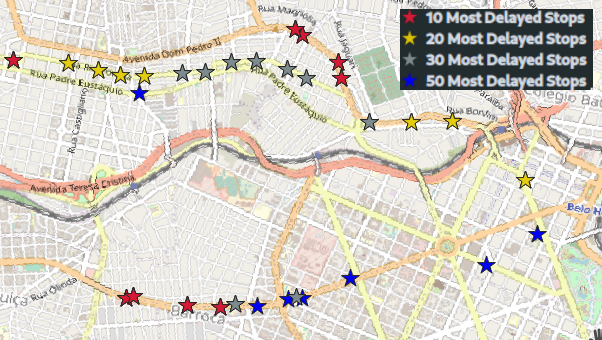
\includegraphics[width=\linewidth]{images/10-50MostDelayedStops.png}
                \end{figure}
        \end{columns}
\end{frame}
\begin{frame}{Delay Analysis}
        \begin{block}{Three Most Delayed Stops for Weekdays}
                \begin{enumerate}
                        \item $\#14793268$ - \textit{Avenida Dom Pedro II 1520} with $7,309$ delays 
                        \item $\#14791617$ - \textit{Avenida Amazonas 7309} with $7,009$ delays
                        \item $\#14790997$ - \textit{Avenida Dom Pedro II 1980} with $6,692$ delays 
                \end{enumerate}
        \end{block}
        \begin{block}{Constants} 
                \begin{enumerate}
                        \item \textit{Global Ahead Average}: $13.42$ minutes 
                        \item \textit{Global Delay Average}: $20.49$ minutes 
                \end{enumerate}
        \end{block}
\end{frame}
\begin{frame}{Delay Analysis}
        \begin{columns}
                \column{0.5\textwidth}  		
        \begin{block}{Stops $\#14793268$ and $\#14790997$} 
                \begin{itemize}
                        \item \textbf{462} meters 
                        \item \textbf{2,590} trips 
                \end{itemize}
        \end{block}
        \begin{block}{\textit{Local Out-Of-Schedule Average}} 
                \begin{itemize}
                        \item $\#14793268$: $19.29$ minutes 
                        \item $\#14790997$: $19.68$ minutes 
                \end{itemize}
        \end{block}
                \column{0.5\textwidth}
                \begin{figure}[t]
                        \centering
                        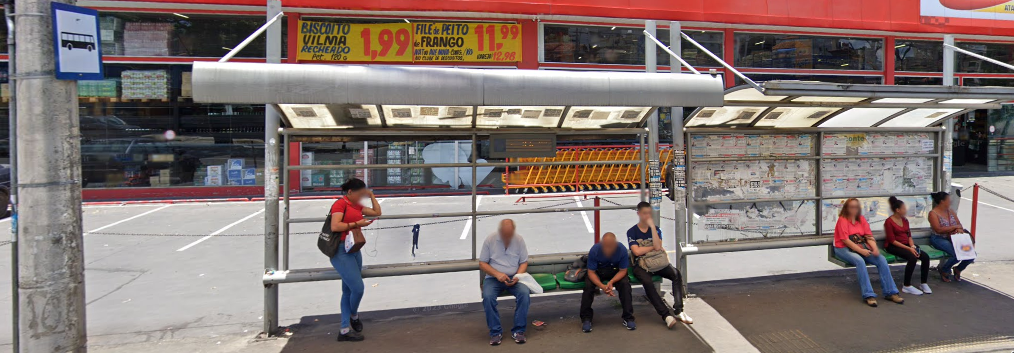
\includegraphics[width=\linewidth]{images/bustop1_pedroii.png}
                \end{figure}
                \begin{figure}[t]
                        \centering
                        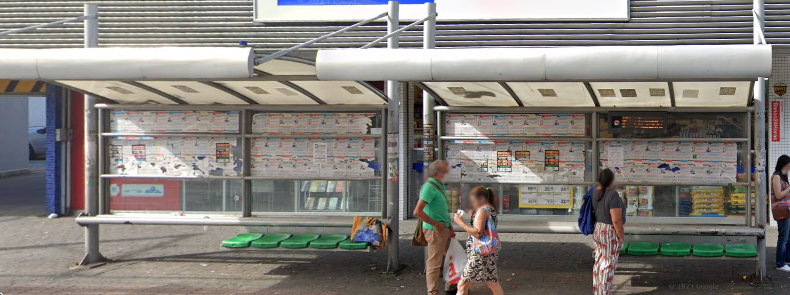
\includegraphics[width=\linewidth]{images/bustop2_pedroii.png}
                \end{figure}
        \end{columns}
\end{frame}
\begin{frame}{Delay Analysis}
        \begin{figure}[H]
                \centering
                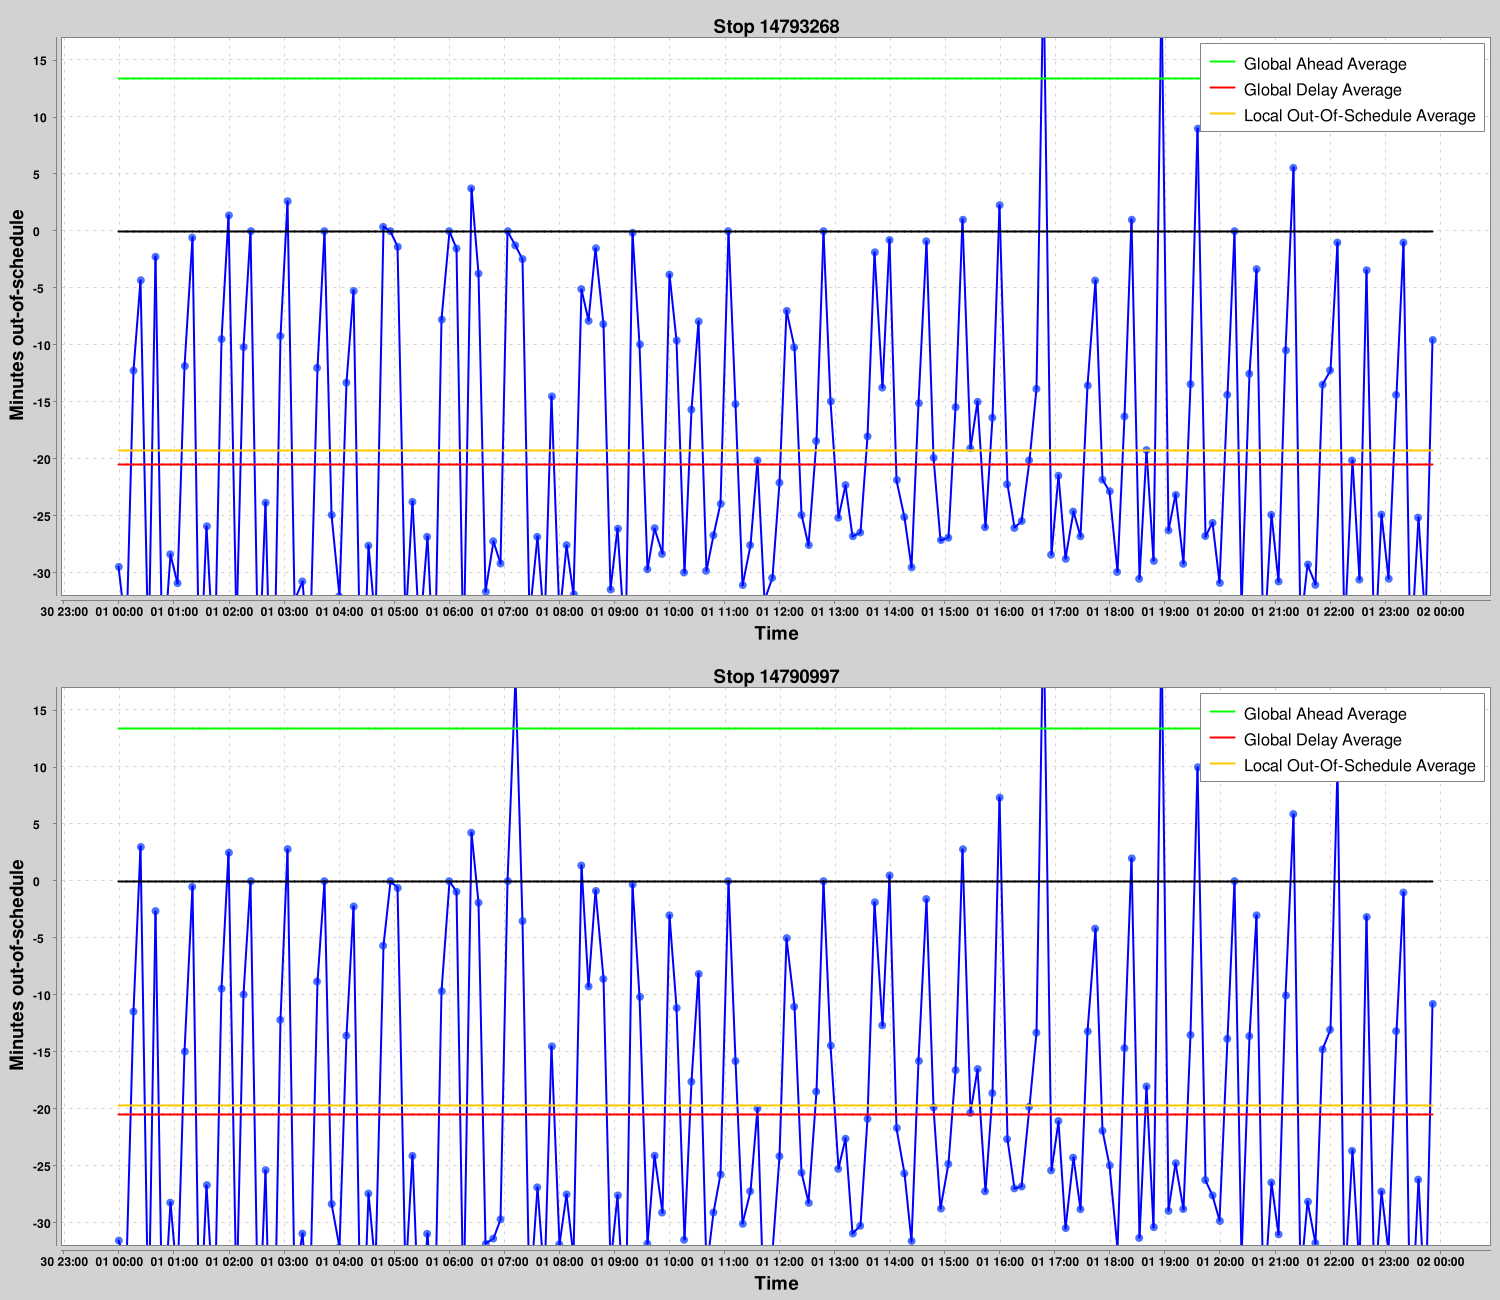
\includegraphics[height=6.5cm,width=10cm]{images/stops2.png}
        \end{figure}
\end{frame}

\subsection{Comparison Between Generated and Real Data}
\begin{frame}{Comparison Between Generated and Real Data}
        \begin{block}{Overview} 
                The previous analysis was only possible because Belo Horizonte's GTFS defines the expected time for all bus stops on every trip. The \textit{Trip Expected Time Generator} generates the expected times when missing, so, we executed this component with Belo Horizonte's data and compared the expected times generated
with those defined at the GTFS.
        \end{block}
\end{frame}
\begin{frame}{Comparison Between Generated and Real Data}
        \begin{columns}
                \column{0.5\textwidth}  		
                \begin{block}{Trip entirely out of schedule} 
                        \begin{itemize}
                                \item GTFS: 78,291 
                                \item Generated: 75,073 
                                \item \textbf{Diff}: 3,218 (\textbf{4.29\%})
                        \end{itemize}
                \end{block}
                \begin{block}{Trips with departure \textbf{or} arrival on time} 
                        \begin{itemize}
                                \item GTFS: 54,122 
                                \item Generated: 54,271 
                                \item \textbf{Diff}: 149 (\textbf{0.27\%}) 
                        \end{itemize}
                \end{block}
                \column{0.5\textwidth}
                \begin{block}{Trip entirely on time} 
                        \begin{itemize}
                                \item GTFS: 4
                                \item Generated: 0 
                                \item \textbf{Diff}: 4 (\textbf{100\%}) 
                        \end{itemize}
                \end{block}
                \begin{block}{Trips with departure \textbf{and} arrival on time} 
                        \begin{itemize}
                                \item GTFS: 475 
                                \item Generated: 596
                                \item \textbf{Diff}: 121 (\textbf{25.47\%})
                        \end{itemize}
                \end{block}
        \end{columns}
\end{frame}
\begin{frame}{Comparison Between Generated and Real Data}
        \begin{table}[h!]
                \centering
                \begin{tabular}{|c|c|c|r|r|}
                        \hline
                        \multicolumn{3}{|c|}{} &   GTFS  &  Generated  \\
                        \hline
                        \multirow{3}{*}{Weekday} & \multicolumn{2}{|c|}{$ON\_TIME$} & $3.3\%$ & $3.2\%$ \\\cline{2-5}
                                                 & \multicolumn{2}{|c|}{$AHEAD\_OF\_SCHEDULE$} & $6.9\%$ & $17.8\%$ \\\cline{2-5}
                                                 & \multicolumn{2}{|c|}{$DELAYED$} &$89.8\%$ & $79.0\%$  \\
                                                 \hline
                        \multirow{3}{*}{Saturday} & \multicolumn{2}{|c|}{$ON\_TIME$} & $3.9\%$ & $3.5\%$ \\\cline{2-5}
                                                  & \multicolumn{2}{|c|}{$AHEAD\_OF\_SCHEDULE$} & $6.5\%$ & $18.4\%$ \\\cline{2-5}
                                                  & \multicolumn{2}{|c|}{$DELAYED$} &$89.6\%$ & $78.1\%$  \\
                                                  \hline
                        \multirow{3}{*}{Sunday} & \multicolumn{2}{|c|}{$ON\_TIME$} & $4.4\%$ & $3.9\%$ \\\cline{2-5}
                                                & \multicolumn{2}{|c|}{$AHEAD\_OF\_SCHEDULE$} & $5.4\%$ & $18.5\%$ \\\cline{2-5}
                                                & \multicolumn{2}{|c|}{$DELAYED$} &$90.2\%$ & $77.6\%$  \\
                                                \hline
                \end{tabular}
        \end{table}
\end{frame}
\begin{frame}{Comparison Between Generated and Real Data}
        \begin{columns}
                \column{0.5\textwidth}  		
                \begin{block}{Global Averages} 
                        \begin{itemize}
                                \item \textit{Global Ahead Average} 
                                        \begin{itemize}
                                                \item GTFS: $13.42$ minutes 
                                                \item Generated: $38.57$ minutes 
                                                \item \textbf{Diff}: $25.15$ minutes 
                                        \end{itemize}
                                \item \textit{Global Delay Average} 
                                        \begin{itemize}
                                                \item GTFS: $20.49$ minutes 
                                                \item Generated: $24.75$ minutes 
                                                \item \textbf{Diff}: $4.26$ minutes 
                                        \end{itemize}
                        \end{itemize}
                \end{block}
                \column{0.5\textwidth}
                \begin{block}{\textit{Local Out-Of-Schedule Average}} 
                        \begin{itemize}
                                \item $\#14793268$
                                        \begin{itemize}
                                                \item GTFS: $19.29$ minutes 
                                                \item Generated: $15.54$ minutes 
                                                \item \textbf{Diff}: $3.75$ minutes 
                                        \end{itemize}
                                \item $\#14790997$ 
                                        \begin{itemize}
                                                \item GTFS: $19.68$ minutes 
                                                \item Generated: $14.68$ minutes 
                                                \item \textbf{Diff}: $5$ minutes 
                                        \end{itemize}
                        \end{itemize}
                \end{block}
        \end{columns}
\end{frame}


\subsection{Limitations}
\begin{frame}{Limitations}
        \begin{block}{Limitations}
                The {\em Real-Time Data Collector} is the most fragile component due
                to the third-party real-time traffic API interface.
                \begin{itemize}
                        \item Size and quality of the data
                        \item Scheduled routes with no entries reported
                                \begin{enumerate}
                                        \item \textit{720 - Circular Saúde MG20} missed $175$ trips
                                        \item \textit{912 - Conjunto Taquaril/Praça Che Guevara} missed $210$ trips
                                \end{enumerate}
                \end{itemize}

        \end{block}
\end{frame}

\section{Conclusion}
\begin{frame}{Conclusion}
        \begin{block}{Concluding Remarks}
                \begin{itemize}
                        \item Delays in Belo Horizonte follow a {\em log-normal} distribution
                        \item Analysis using data generated with the \textit{Trip Expected Time Generator}
                        \item \textit{PondiônsTracker} as a viable option when GTFS-RT is unavailable
                \end{itemize}
        \end{block}
        \begin{block}{Future Work}
                \begin{itemize}
                        \item Futher explore Belo Horizonte Public Transportation Network using deep learning for graphs approaches 
                        \item Reproduce Belo Horizonte's results with other cities
                \end{itemize}
        \end{block}
\end{frame}

\bibliography{ref}

\begin{frame}{Conclusion}
        Thanks!!
                \begin{figure}[H]
                        \centering
                        
\includegraphics[scale=0.20]{images/thanks.png}
                \end{figure}
\end{frame}
\end{document}
